\chapter{Lab 1 - Setting Up the Development Environment}

In this lab, we'll set up the basic development environment for the rest of our labs. Firstly
I'll introduce you to the tools and we'll install them, then we'll compile MOS, run it in QEMU
for the first time, and then attach GDB to it.

Finally, and hopefully, you can get your favorite IDE set up to work with MOS.

\section{Introduction to the Tools}

MOS is an operating system, thus, preparing for a development environment is already not
an easy task (bruh). Several efforts have been made to make the process easier.

We are currently targeting the 32-bit \texttt{x86} architecture, the tools in table \ref{tab:tools}
are the ones we'll be using.

\begin{table}[h!]
    \centering
    \begin{tabular}{|l|c|c|}
        \hline \textbf{Tool}               & \textbf{Description}     & \textbf{Installation}            \\
        \hline \texttt{CMake}              & \ref{sec:cmake}          & \ref{sec:cmake-install}          \\
        \hline \texttt{i686-elf} toolchain & \ref{sec:cross-compiler} & \ref{sec:cross-compiler-install} \\
        \hline \texttt{NASM}               & \ref{sec:nasm}           & \ref{sec:nasm-install}           \\
        \hline \texttt{cpio}               & \ref{sec:cpio}           & \ref{sec:cpio-install}           \\
        \hline \texttt{qemu-system-i386}   & \ref{sec:qemu}           & \ref{sec:qemu-install}           \\
        \hline
    \end{tabular}
    \caption{Tools used in this lab}
    \label{tab:tools}
\end{table}

\subsection{CMake} \label{sec:cmake}

\begin{quote}
    CMake is an open-source, cross-platform family of tools designed to build, test and package
    software\footnote{https://cmake.org/}
\end{quote}

MOS uses CMake as the build system generator, it supports many build systems like `Make', `Ninja',
`Visual Studio' and `Xcode'.

\begin{note}
    \item It's the actual build system (e.g. `Make') that starts the compiler, linker, etc.,
    CMake is only to \textbf{generate} the configuration files for such build system.
\end{note}

We'll use `Make' as the build system for MOS in this tutorial, but
\textbf{you can use `Ninja' if you want}.

\subsection{NASM} \label{sec:nasm}

NASM is an assembler for x86 architecture. There are several files under `arch/x86`
that are written in NASM. It has a cleaner syntax than the GNU assembler (i.e. \texttt{as}).

\subsection{cpio} \label{sec:cpio}

Cpio is the format of an archive, and also the tool to create such archives. MOS uses cpio as
the initial root filesystem.

\subsection{qemu-system-i386} \label{sec:qemu}

QEMU is an open-source emulator, it also provides a gdb stub for debugging. It can be
installed via your Linux's package manager.

(e.g. \texttt{apt install qemu-system-i386} or \texttt{pacman -S qemu-system-x86}, \dots).

See its \href{https://www.qemu.org/download}{download page} for more details.

\subsection{i686-elf Toolchain} \label{sec:cross-compiler}

As its name suggests, this is a cross toolchain for `i686-elf' target. `i686' means the 32-bit
x86 architecture, and `elf' is the executable format. They together form the `target-triple' of
the toolchain.

\begin{tip}
    \item Most 64-bit Linux OSes have `target triple' of \texttt{x86\_64-pc-linux-gnu}, or
    \texttt{x86\_64-linux-gnu}.
    \item Read more about `target triple' at \url{https://wiki.osdev.org/Target_Triplet}.
\end{tip}

Unlike other applications (e.g. \texttt{bash} or \texttt{vim}) that they run on an existing
operating system and a standard C library (say, \texttt{glibc} or \texttt{musl}). MOS itself is
the operating system, thus there's not an existing OS for it to run on, neither a standard libc
(i.e. no \texttt{printf}, no \texttt{malloc} etc.) for it to use, considering you're directly
interacting with the CPU and the hardware.

This is called `bare-metal' environment, or `freestanding' environment, a `bare-metal' compiler
toolchain is exactly for this situation.

\begin{warning}
    \item One should never use a hosted compiler (e.g. the \texttt{gcc} installed on the lab machine)
    to cross-compile for a bare-metal environment when they are targeting a different architecture,
    (\texttt{x86} and \texttt{x86\_64} are different), it \textit{\textbf{may sometimes}} work, but
    you'll have to add a lot of unnecessary flags.

    \item See \url{https://wiki.osdev.org/Why_do_I_need_a_Cross_Compiler%3F} for more information.
\end{warning}

\section{Installating the Tools}

\subsection{CMake} \label{sec:cmake-install}

CMake should come with your Linux distribution's package manager, MOS requires at least version
3.20, but any newer version is recommended.

\subsection{NASM} \label{sec:nasm-install}

NASM can be installed via your Linux's package manager, the minimum version of NASM tested is
\texttt{2.15.03}. A pre-built binary from \href{https://www.nasm.us}{NASM's website} is also
available.

\subsection{cpio} \label{sec:cpio-install}

cpio can also be installed via your Linux's package manager, the minimum version of cpio
tested is \texttt{2.12}.

\subsection{qemu-system-i386} \label{sec:qemu-install}

TODO

\subsection{i686-elf Toolchain} \label{sec:cross-compiler-install}

Installing the cross-compiler toolchain is probably the most difficult part of this lab,
but it's once and for all, you don't have to do it again (unless you want to upgrade the
toolchain).

There are majorly two ways to get this toolchain, either by building it from source or by
downloading a pre-built binary.

\subsubsection{Downloading a pre-built binary}

If you don't want to build the toolchain from source, you can download a pre-built
binary from
\href{https://github.com/moodyhunter/i686-elf-prebuilt/releases}{moodyhunter/i686-elf-prebuilt}
(choose the i686 one).

\begin{warning}
    \item Using pre-built binary saves time, but please consider doing so \textbf{only} if
    you trust the author.
    \item The above pre-built binary is built with GitHub Actions, and is built on Ubuntu 20.04.5
    LTS (Image \texttt{ubuntu-20.04} version \texttt{20221027.1}).
\end{warning}

\subsubsection{Building From Source}

The source code of binutils and gcc can be found at
\href{https://www.gnu.org/software/binutils}{GNU Binutils's Website} and
\href{https://gcc.gnu.org}{GNU GCC's Website} respectively.

\begin{note}
    \item For Arch Linux users, checkout
    \href{https://github.com/moodyhunter/repo/blob/main/moody/i686-elf-binutils/PKGBUILD}{i686-elf-binutils},
    \href{https://github.com/moodyhunter/repo/blob/main/moody/i686-elf-gcc/PKGBUILD}{i686-elf-gcc} and
    \href{https://github.com/moodyhunter/repo/blob/main/moody/i686-elf-gdb/PKGBUILD}{i686-elf-gdb}.
\end{note}

The script located at \texttt{docs/assets/i686-elf-toolchain.sh} can download, compile and
install the toolchain into the directory specified by the \texttt{PREFIX} variable.

\section{Building MOS}

\begin{note}
    \item Before you continue reading, make sure \texttt{i686-elf-gcc}, \texttt{i686-elf-ld},
    \texttt{nasm}, \texttt{cpio} are in your \texttt{PATH}.
\end{note}

\subsection{Cloning the Repository}

The recommended way to get MOS is to clone the repository from GitHub:

\begin{verbatim}
    git clone https://github.com/moodyhunter/MOS
    cd MOS
\end{verbatim}

\subsection{Configuring MOS}

If you have a correct setup, then configuring step should be as simple as:

\begin{verbatim}
    $ mkdir build && cd build
    $ cmake ..
\end{verbatim}

The first line creates a build directory, we are not going to build MOS in the source directory
directly, because there will be many generated files, and it's not a good idea to pollute the
source directory.

The second line runs CMake to configure MOS, after running this command, you should see a
bunch of output, similar to \ref{fig:cmake-output}.

\begin{figure}[h]
    \centering
    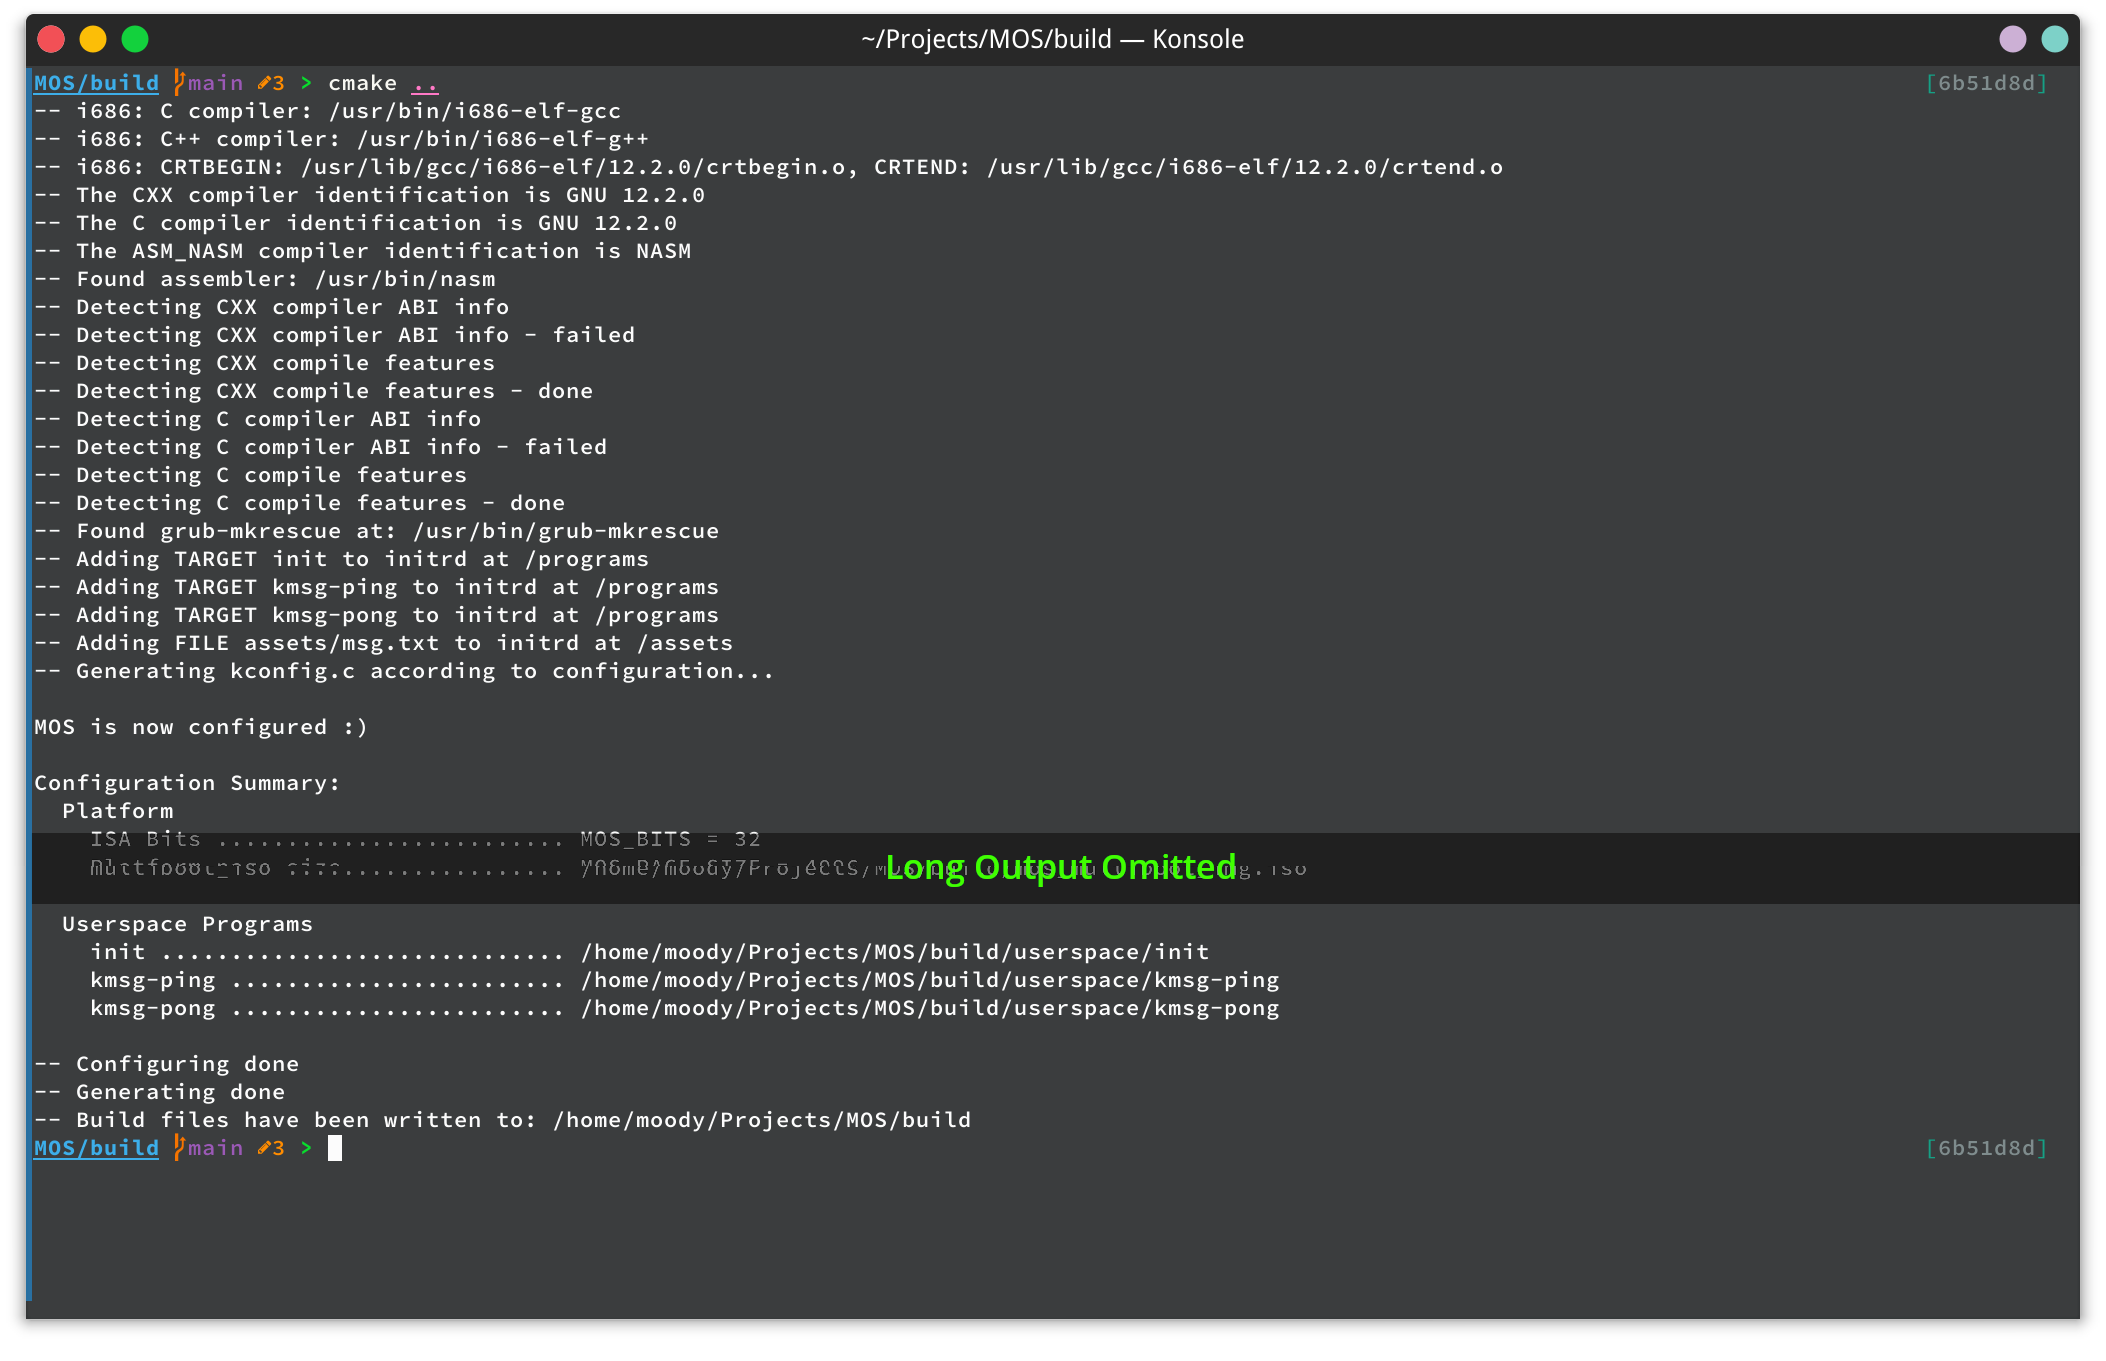
\includegraphics[width=\textwidth]{assets/c1.mos-cmake-configure.png}
    \caption{CMake Output}
    \label{fig:cmake-output}
\end{figure}

\begin{note}
    \item Don't worry if you see \texttt{Detecting C compiler ABI info} and
    \texttt{Detecting CXX compiler ABI info} fails, it's because CMake doesn't know what to do
    with a freestanding compiler, thus this check is meaningless.

    \item You may also see \texttt{grum-mkrescue} is not found, don't worry as well :), we are
    not going to use it.
\end{note}

If you don't see the \texttt{-- Configuring done} or \texttt{-- Generating done} line, then
something has been wrong, and you should scroll up and see what's wrong.

\begin{tip}
    \item The \texttt{build} directory is where all the generated files are located, you can
    safely delete it and re-run CMake to re-generate the files, in case you messed up something.
\end{tip}

\subsection{Building MOS}

After configuring MOS, you can build MOS by running \texttt{make}.

This command will only build the core part of MOS, which is the kernel and the userspace library.
See the table below for the list of targets:

\begin{table}[h]
    \centering
    \small
    \begin{tabular}{|l|l|l|}
        \hline
        \textbf{Target}                   & \textbf{Description}               & \textbf{Dependencies}                                \\ \hline
        \texttt{all} \textit{(default)}   &                                    & \texttt{mos\_kernel.elf}, \texttt{mos\_libuserspace} \\ \hline
        \texttt{mos\_kernel.elf}          & Bare kernel without booting        & \textit{None}                                        \\ \hline
        \texttt{mos\_libuserspace}        & Userspace standard library         & \texttt{mos\_kernel.elf}                             \\ \hline
        \texttt{multiboot}                & \texttt{multiboot} bootable kernel & \texttt{mos\_kernel.elf}                             \\ \hline
        \texttt{mos\_initrd}              & Initrd image                       & \texttt{mos\_userspace\_programs}                    \\ \hline
        \texttt{mos\_userspace\_programs} & Userspace programs                 & \texttt{init}, \texttt{kmsg-ping}, \dots             \\ \hline
        \texttt{init}                     & The init program                   & \texttt{mos\_libuserspace}                           \\ \hline
        \texttt{kmsg-ping}                & A program to test kernel IPC       & \texttt{mos\_libuserspace}                           \\ \hline
        \dots                             & \dots                              & \dots                                                \\ \hline
    \end{tabular}
    \caption{Targets}
    \label{tab:targets}
\end{table}

We are going to build the \texttt{multiboot} and \texttt{mos\_initrd} targets, which are the two
meta targets that 1) produce a bootable kernel and 2) build and package the initrd image.

So the command will be \texttt{make multiboot mos\_initrd}.

You'll then see two files being generated in the \texttt{build} directory:

\begin{itemize}
    \item \texttt{mos\_multiboot.bin} is the kernel image, which is a multiboot-compliant kernel.
    \item \texttt{initrd.cpio} is the initrd image, which contains the userspace programs.
\end{itemize}

Several other files are also generated, for more information, read the MOS documentation at \href{TODO}{TODO}.

\section{Running MOS}

Once we have compiled MOS, we can run it in QEMU.

The command passed to QEMU will be flexible based on your needs, but the most basic command is:

\begin{verbatim}
    qemu-system-i386 -kernel mos_multiboot.bin -initrd initrd.cpio
\end{verbatim}

You can pass more arguments to QEMU:

\begin{itemize}
    \item \texttt{-s} to enable the QEMU GDB stub, which allows you to debug MOS using GDB.
    \item \texttt{-S} to pause the CPU before starting up, which allows GDB to take control of
          the booting process.
    \item \texttt{-m} to specify the amount of RAM to be allocated to the VM (say \texttt{-m 512M}).
    \item \texttt{-serial stdio} to redirect the serial output to your terminal, in the early stage
          of booting, MOS prints lots of information to the serial port to help you debug.
    \item \texttt{-append} to pass arguments to the kernel, for a list of supported arguments,
          see the MOS documentation at \href{TODO}{TODO}.
\end{itemize}

\section{Debugging MOS}

After successfully building and running MOS, you may want to debug it (just in case your code crashes
the kernel).

\subsection{Required QEMU Arguments} \label{sec:qemu-args}

As mentioned above, we need to pass 2 more arguments \texttt{-s} and \texttt{-S} to QEMU so that it 1) enables the GDB stub, and
2) pauses the CPU before starting up (so that we have time to attach and place breakpoints).

After adding these two arguments, when starting up QEMU, you will see a message like Figure
\ref{fig:qemu-gdb-paused}.

\begin{figure}[h]
    \centering
    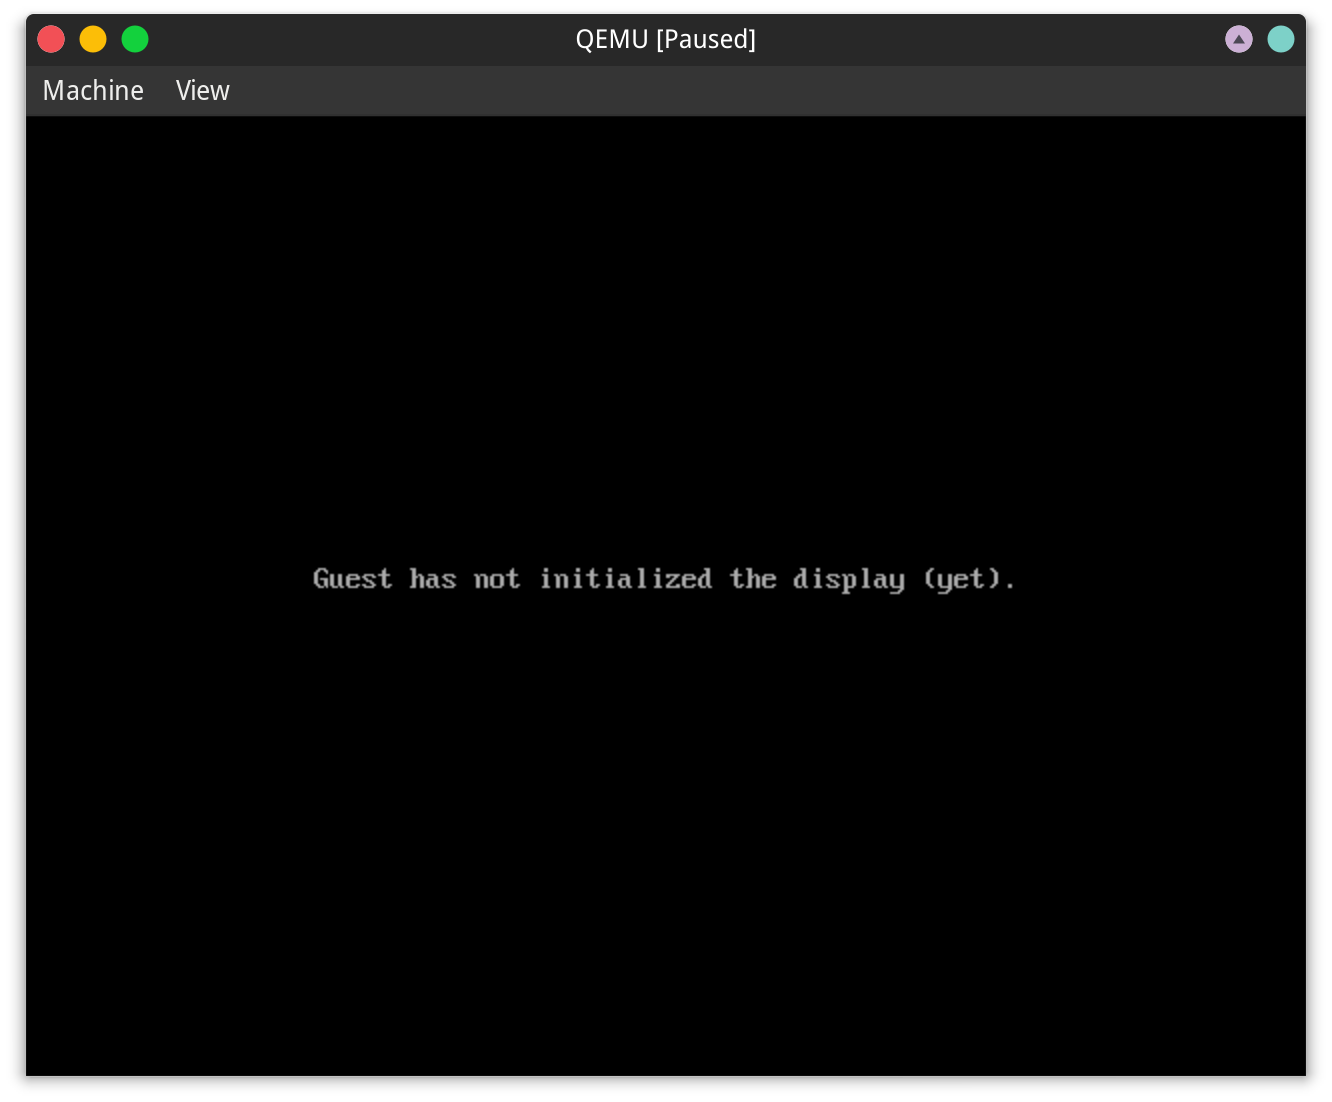
\includegraphics[width=\textwidth]{assets/c1.mos-qemu-gdb-paused.png}
    \caption{QEMU GDB in Paused State}
    \label{fig:qemu-gdb-paused}
\end{figure}

This means that QEMU is waiting for a GDB connection, and we can now continue to the next step.

\subsection{Configuring GDB} \label{sec:gdb-config}

Note that we are targeting the \texttt{i686-elf} architecture, so you should use \texttt{i686-elf-gdb}
instead of \texttt{gdb}.

To begin with, we need to tell GDB where the kernel image file is, so that it can load the symbols
and debug information from it.

You've probably already seen a \texttt{gdbinit} file in the \texttt{build} directory. This file
contains commands for GDB to recognize our userspace programs, we'll pass this file to GDB using
the \texttt{-x} argument.

So the overall command will be:

\begin{verbatim}
    cd /PATH/TO/MOS/build
    i686-elf-gdb ./mos_multiboot.bin -x ./gdbinit
\end{verbatim}

\subsection{Attaching to QEMU} \label{sec:gdb-attach}

After GDB starts, you'll see it's `adding symbol table from file' thanks to our \texttt{gdbinit} file.
Now we need to attach GDB to QEMU, so that we can place breakpoints and debug the kernel.

QEMU (by default) listens on port 1234 for GDB connections, so we need to tell GDB to connect to it:

\begin{verbatim}
    (gdb) target remote localhost:1234
\end{verbatim}

GDB will then connect to QEMU, and you'll see a message like Figure \ref{fig:gdb-attached}.

\begin{figure}[h]
    \centering
    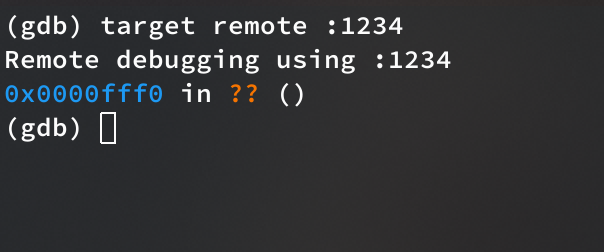
\includegraphics[width=\textwidth]{assets/c1.gdb-attached.png}
    \caption{GDB Attached to QEMU}
    \label{fig:gdb-attached}
\end{figure}

Try typing \texttt{break main} and then \texttt{continue} to see if it pauses at the \texttt{main}
function, you should see a message like Figure \ref{fig:gdb-paused}.

\begin{figure}[ht]
    \centering
    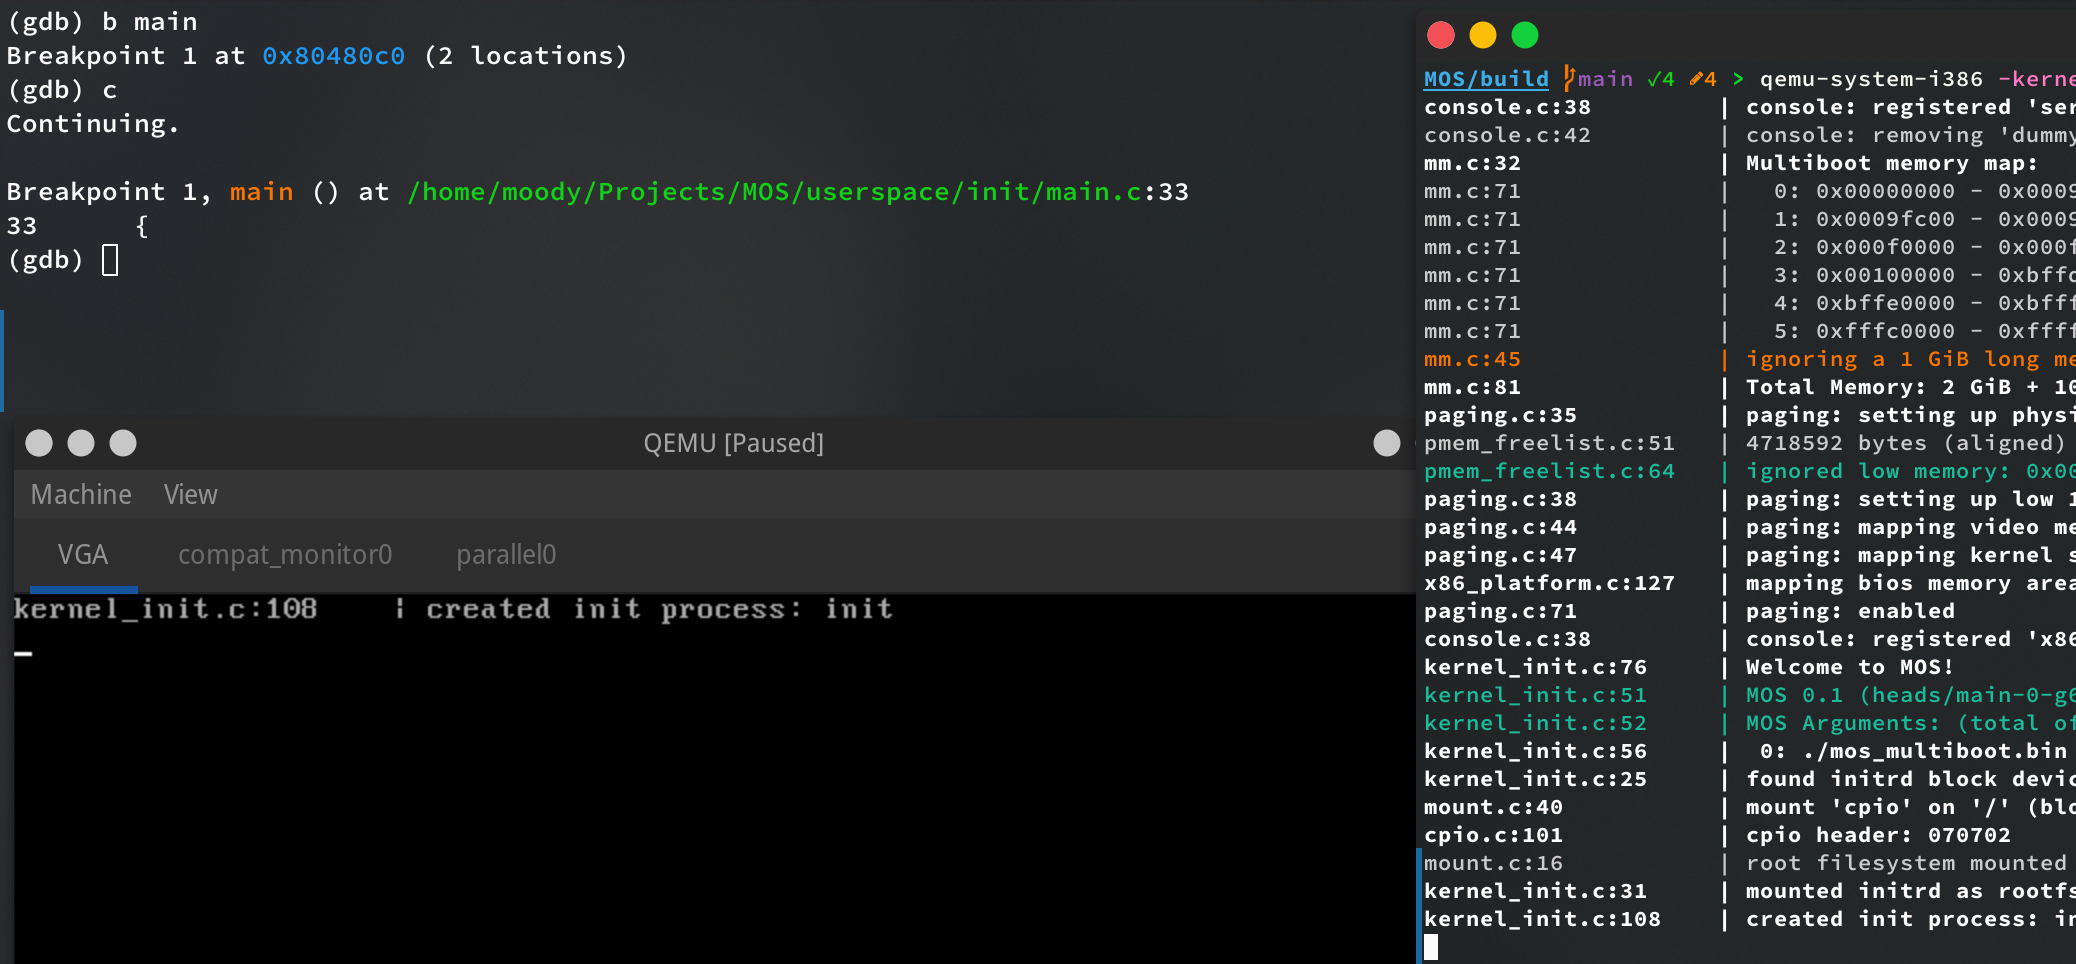
\includegraphics[width=\textwidth]{assets/c1.gdb-paused.png}
    \caption{GDB Paused at \texttt{main}}
    \label{fig:gdb-paused}
\end{figure}

\subsection{Configure your IDE for Future Debugging} \label{sec:ide-config}

\begin{note}
    \item Since I'm personally using VSCode, only the VSCode part will be covered here. If you are
    using any other IDE (e.g. CLion), things \textbf{may} be different, but the underlying idea
    of remote debugging should be the same.

    \item IDEs are updating very fast, so the screenshots \textbf{may} be outdated. Ask me if you
    have any questions.
\end{note}

As you may (or may not) realize, attaching GDB to QEMU is basically the process of `remote debugging',
So we can configure our IDE to do this automatically, with the only two exceptions being that
1) the GDB in use is our \texttt{i686-elf-gdb} instead of the default \texttt{gdb} and 2) we need to
specify the \texttt{gdbinit} file.

\subsubsection{Prepared VSCode Setup} \label{sec:vscode-config}

To use a prepared setup for VSCode, see the \texttt{launch.json} file in the \texttt{.vscode}
directory, which is also my personal configuration for debugging MOS.

Install \texttt{tmux} on your machine and press \texttt{F5}, a QEMU window will pop up and you'll see the kernel booting up, with the breakpoints
you set in your IDE as shown in Figure \ref{fig:vscode-debugging}.

In this setup, you can also use \texttt{tmux attach-session -t mos\_kernel\_debug} to attach to the serial
port.

\begin{figure}[ht]
    \centering
    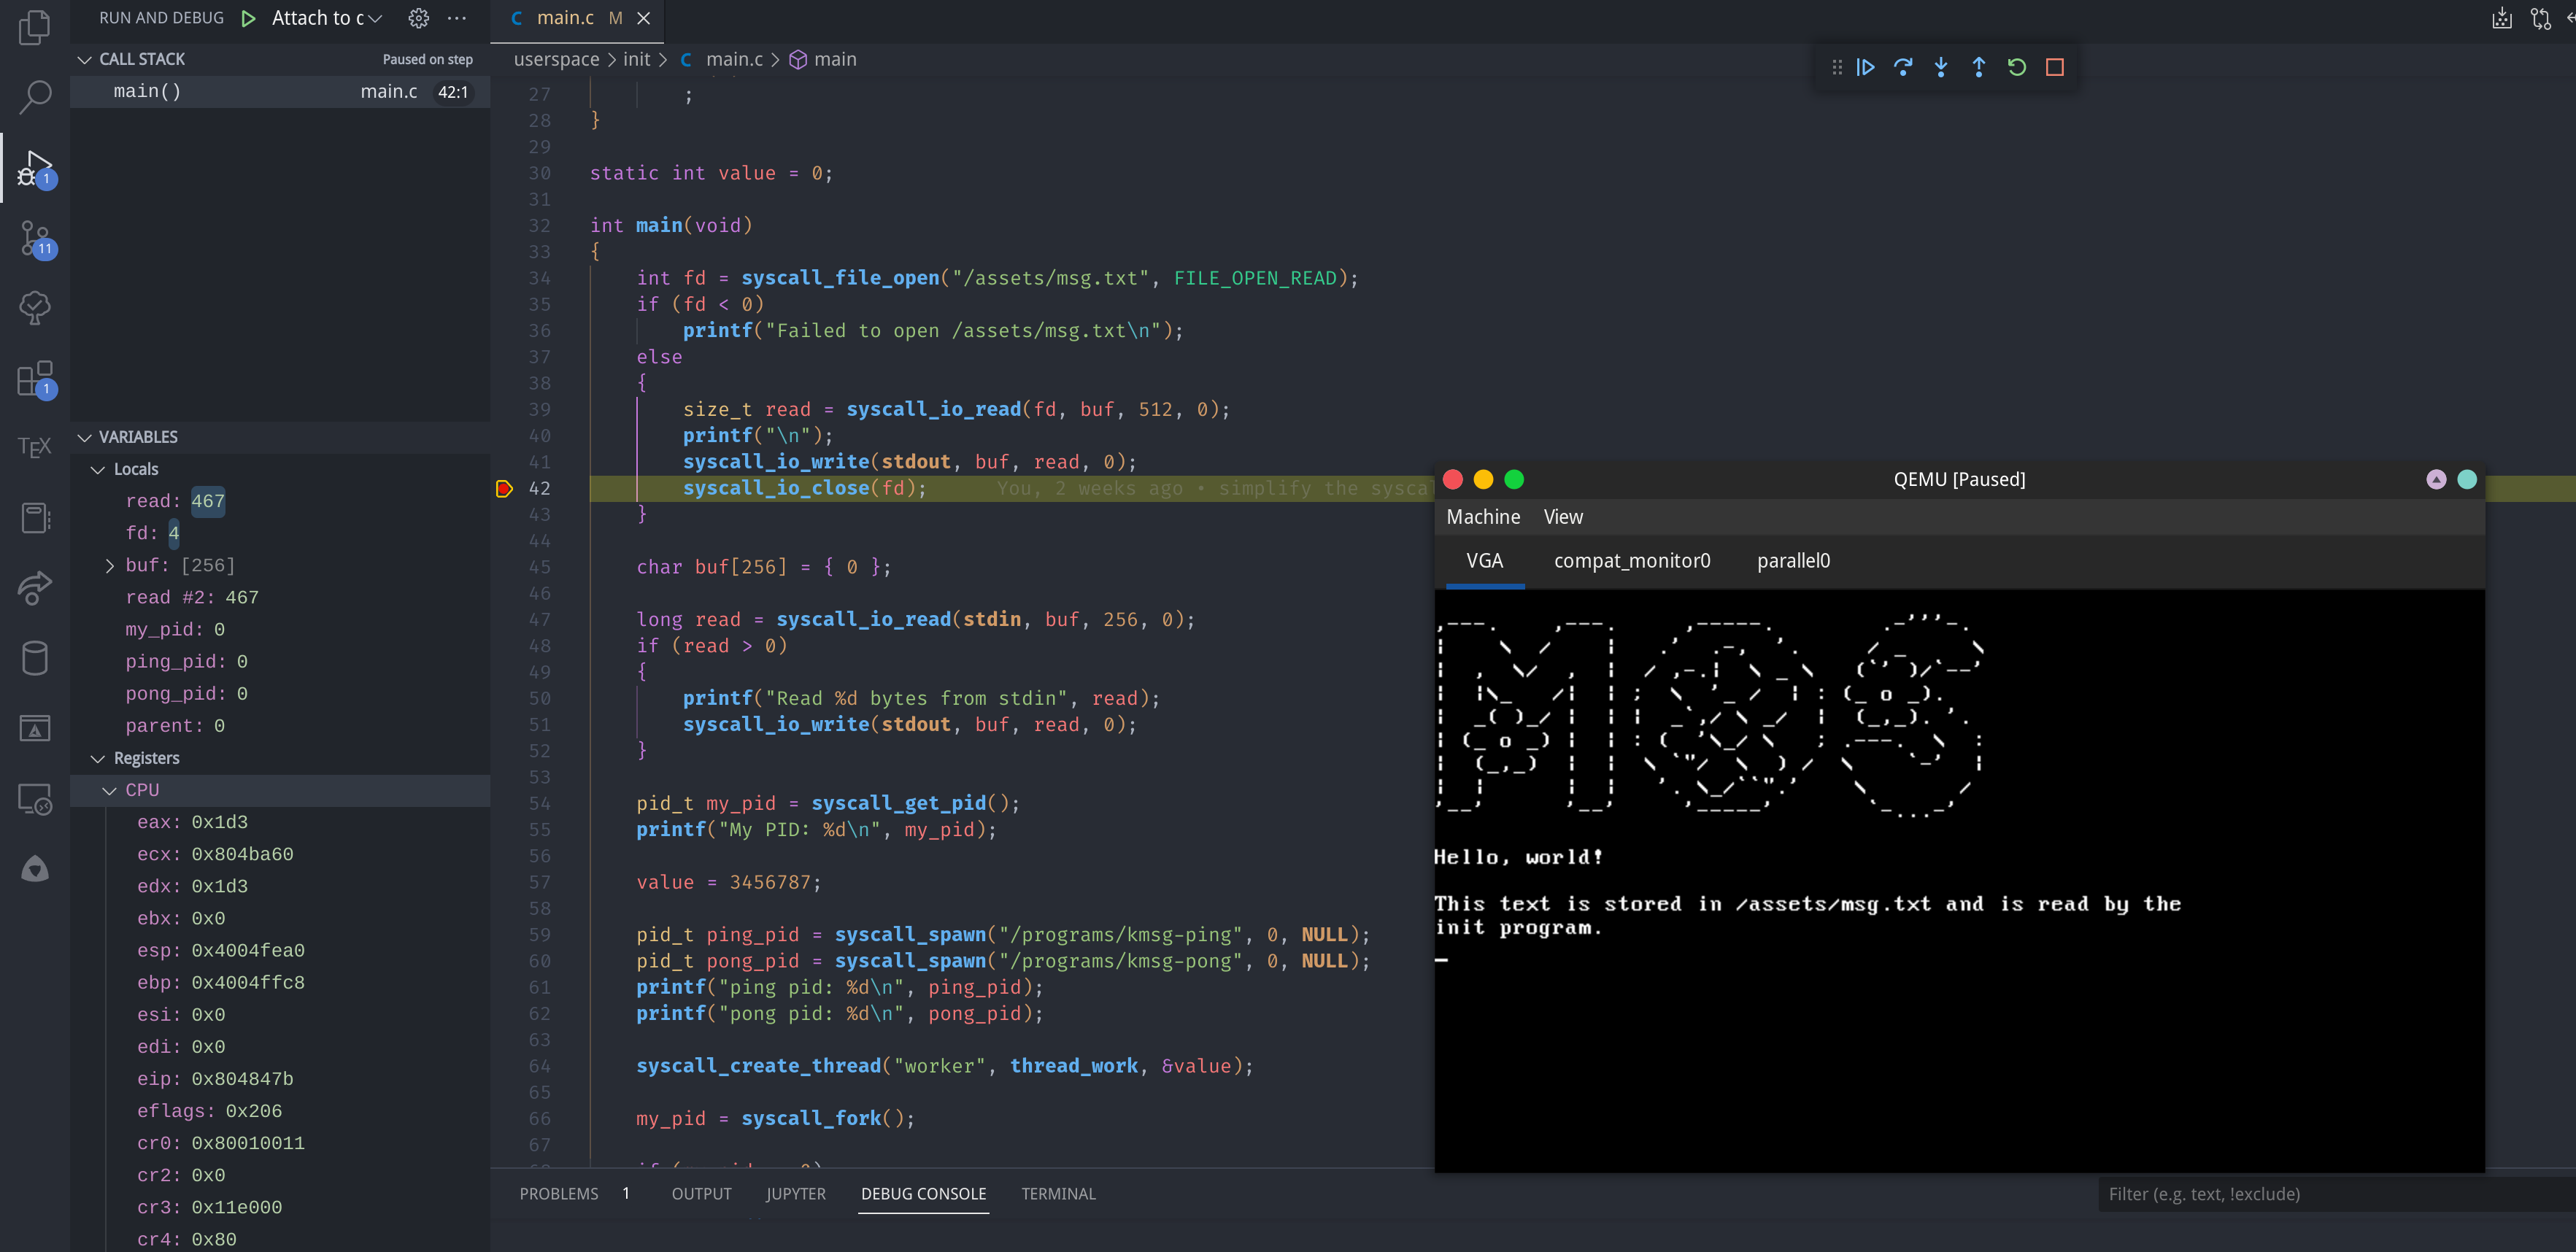
\includegraphics[width=\textwidth]{assets/c1.vscode-debugging.png}
    \caption{VSCode Debugging MOS}
    \label{fig:vscode-debugging}
\end{figure}

\begin{exercise}
    \item In the \texttt{mos\_start\_kernel} function (in \texttt{kernel/kernel\_init.c}), add some code
    to print out your name with some other information. e.g. `This is Moody's own version of MOS!'

    Compile and run the kernel, do you see your name printed out?

    \begin{mdframed}
        Hint: There are various ways to print out strings in MOS kernel, you can either of:
        \texttt{printk}, \texttt{pr\_info}, \texttt{pr\_info2}, \texttt{pr\_emph}, \texttt{pr\_warn},
        \texttt{pr\_emerg} or \texttt{pr\_fatal}.
    \end{mdframed}

    Can you spot the differences between these functions?

    \item You can find a call to \texttt{cmdline\_get\_init\_path} in \texttt{mos\_start\_kernel} function,
    which returns a string named \texttt{init\_path}. Try writing code to print out this string.

    \begin{mdframed}
        Hint: The above ways of printing out strings have similar usage like \texttt{printf}.
    \end{mdframed}

    \item Try to set a breakpoint somewhere in the \texttt{mos\_start\_kernel} function, start debugging
    the kernel and see if it works.

    \item Try setting another breakpoint in the userspace program, \texttt{init}. The corresponding
    source file is at \texttt{userspace/init/main.c}.
\end{exercise}
